Submitted:

\begin{verbatim}[t4, t3, t2, t1]\end{verbatim}

t1 is a transition of the given Petri net?\begin{quote}Yes.\end{quote}t2 is a transition of the given Petri net?\begin{quote}Yes.\end{quote}t3 is a transition of the given Petri net?\begin{quote}Yes.\end{quote}t4 is a transition of the given Petri net?\begin{quote}Yes.\end{quote}At most 8 steps provided?\begin{quote}Yes.\end{quote}Start marking:

\begin{quote} [(s1,1),(s2,1),(s3,1),(s4,1)] \end{quote}Step 1

 Transition t4 

Intermediate marking (after collecting tokens)

\begin{quote} [(s1,0),(s2,1),(s3,1),(s4,0)] \end{quote}Final marking (after distributing tokens)

\begin{quote} [(s1,0),(s2,2),(s3,1),(s4,1)] \end{quote}

\begin{centering}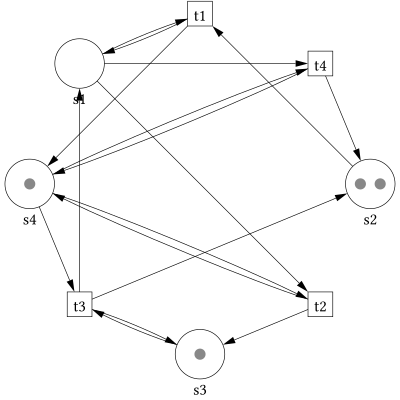
\includegraphics[min width=0.4\textwidth=0.6\textwidth,min height=0.4\textwidth=0.6\textwidth,keepaspectratio,max width=0.9\textwidth,max height=0.9\textwidth]{60/graph1petribff5ee5e2d580dc324d906b928cb642fdb23021043dc0552cc786557cea786f011013.pdf}\end{centering}

Step 2

 Transition t3 

Intermediate marking (after collecting tokens)

\begin{quote} [(s1,0),(s2,2),(s3,0),(s4,0)] \end{quote}Final marking (after distributing tokens)

\begin{quote} [(s1,1),(s2,3),(s3,1),(s4,0)] \end{quote}

\begin{centering}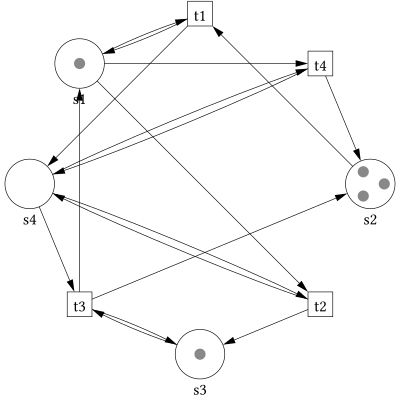
\includegraphics[min width=0.4\textwidth=0.6\textwidth,min height=0.4\textwidth=0.6\textwidth,keepaspectratio,max width=0.9\textwidth,max height=0.9\textwidth]{60/graph2petri07107e2f08eebcc8d629bc02f413fee5db0690a05d28ba7f397f45a479d1469d11013.pdf}\end{centering}

Step 3

 Transition t2 

Intermediate marking (after collecting tokens)

\begin{quote} [(s1,0),(s2,3),(s3,1),(s4,-1)] \end{quote}Contains negative token count (transition was not activated)!

A correct solution is:\begin{verbatim}[t3, t1, t3, t1, t1, t4, t1, t4]\end{verbatim}

